% IEEE conference manuscript for the PINN-EV-Battery project.
% Compile on Overleaf with pdfLaTeX. Keep this file beside figures/.
% IMPORTANT: fill the result macros only from the complete three-seed run.
\documentclass[conference]{IEEEtran}
\IEEEoverridecommandlockouts

% Packages from the official IEEE conference template.
\usepackage{cite}
\usepackage{amsmath,amssymb,amsfonts}
\usepackage{iftex}
% Tectonic uses XeTeX for local previews.  Give headings a real bold Times
% face there while preserving the standard IEEEtran body typography.
\ifXeTeX
  \usepackage{fontspec}
  \newfontfamily\headingfont{TeXGyreTermesX-Regular.otf}[
    BoldFont=TeXGyreTermesX-Bold.otf]
\else
  \newcommand{\headingfont}{\rmfamily}
\fi
\usepackage{algorithmic}
\usepackage{graphicx}
\usepackage{stfloats} % enables bottom placement of full-width IEEE figures
\usepackage{textcomp}
\usepackage{xcolor}

% Additional packages required by this manuscript's tables and units.
\usepackage{booktabs}
\usepackage{multirow}
\usepackage{array}
\usepackage{siunitx}
\usepackage{url}
\usepackage{balance}

% Clear heading hierarchy requested for the conference manuscript:
% sections are 12 pt bold, while subsections remain 10 pt bold.
% Use battery_pinn_ieee_conference_strict.tex if a venue requires the
% untouched IEEEtran heading definitions.
\makeatletter
\def\section{\@startsection{section}{1}{\z@}{1.5ex plus 1.5ex minus 0.5ex}%
{0.7ex plus 1ex minus 0ex}{\normalfont\headingfont\large\centering\bfseries}}
\def\subsection{\@startsection{subsection}{2}{\z@}{1.5ex plus 1.5ex minus 0.5ex}%
{0.7ex plus .5ex minus 0ex}{\normalfont\headingfont\normalsize\bfseries}}
\def\subsubsection{\@startsection{subsubsection}{3}{\parindent}{0ex plus 0.1ex minus 0.1ex}%
{0ex}{\normalfont\headingfont\normalsize\bfseries\itshape}}
\makeatother

\def\BibTeX{{\rm B\kern-.05em{\sc i\kern-.025em b}\kern-.08em
    T\kern-.1667em\lower.7ex\hbox{E}\kern-.125emX}}

\graphicspath{{figures/}}
\sisetup{detect-all,table-number-alignment=center}
\newcommand{\modelname}{PC-MP-PINN}

% Set \resultsavailabletrue only after inserting values from
% results/paper_metrics_summary.csv and variation_gap_vs_previous.csv.
\newif\ifresultsavailable
\resultsavailablefalse
\newcommand{\pending}{\textit{pending}}
\newcommand{\DataC}{\pending}
\newcommand{\PriorC}{\pending}
\newcommand{\ProposedC}{\pending}
\newcommand{\DataT}{\pending}
\newcommand{\PriorT}{\pending}
\newcommand{\ProposedT}{\pending}
\newcommand{\DataStress}{\pending}
\newcommand{\PriorStress}{\pending}
\newcommand{\ProposedStress}{\pending}
\newcommand{\DataMass}{\pending}
\newcommand{\PriorMass}{\pending}
\newcommand{\ProposedMass}{\pending}
\newcommand{\DataSpeed}{\pending}
\newcommand{\PriorSpeed}{\pending}
\newcommand{\ProposedSpeed}{\pending}

\title{{\headingfont\bfseries A Physics-Consistent Electrochemical--Thermal PINN with Concentration-Coupled Particle Stress for Lithium-Ion Battery Surrogate Modeling}}

\author{
\IEEEauthorblockN{1\textsuperscript{st} Ms. Sasikala C,
2\textsuperscript{nd} Naresh V,
3\textsuperscript{rd} Mohamed Shaheel A,
4\textsuperscript{th} Kishore J,
5\textsuperscript{th} Kishore P. S.}
\IEEEauthorblockA{\textit{Department of Computer Science and Engineering} \\
\textit{KPR Institute of Engineering and Technology}\\
Coimbatore, Tamil Nadu, India}
}

\begin{document}
\maketitle

\begin{abstract}
Battery surrogates are useful only when their coupled outputs describe the same physical state. A network may fit concentration, temperature, and stress labels separately while violating the concentration--stress relation inside an electrode particle. This work examines that specific failure mode for constant-current discharge. The proposed physics-consistent multiphysics PINN (\modelname) learns negative-particle lithium concentration and a volume-averaged cell temperature as functions of position, time, C-rate, and ambient temperature. Its objective includes solid-diffusion, symmetry, surface-flux, and thermal-energy residuals. Particle stresses are then calculated from the predicted concentration using a spherical linear-elastic operator; they are not independent neural outputs. Reference fields come from PyBaMM SPMe simulations with the Chen2020 parameter set. Evaluation is organized by complete operating conditions and compares three model variants at three label budgets and three random seeds. The reported measures examine prediction error, conservation, peak stress, agreement between electrochemical and mechanical fields, and inference time. The study concerns a discharge surrogate built from simulated data. It does not claim experimental stress validation, cycle aging, state-of-health estimation, or remaining-life prediction.

\end{abstract}

\begin{IEEEkeywords}
physics-informed neural network, lithium-ion battery, SPMe, thermal model, diffusion-induced stress, multiphysics surrogate, sparse data
\end{IEEEkeywords}

\section{Introduction}
An electric-vehicle battery-management system measures current, terminal voltage, and a limited number of temperatures. It cannot directly observe the lithium profile within an active-material particle or the stress caused by that profile. Electrochemical models can estimate these internal variables, although repeated numerical solves become costly when a controller, optimizer, or uncertainty study needs many queries. The Doyle--Fuller--Newman model gives a detailed porous-electrode description \cite{doyle1993dfn}. Reduced formulations, including the single-particle model with electrolyte dynamics (SPMe), trade some spatial detail for lower computational cost \cite{marquis2019spme,richardson2020gspm,planella2022continuum}. A physics-informed neural network offers a different approximation: it fits simulated states while its derivatives are checked against selected governing equations \cite{raissi2019pinn}.

Published battery PINNs already address parameter recovery, electrochemical surrogates, temperature prediction, and health estimation \cite{hassanaly2024part1,hassanaly2024part2,wang2023temperature,wang2024parameter}. Electrochemical, thermal, and mechanical terms in one model are therefore not sufficient evidence of novelty. Wei \emph{et al.}, for example, combine those domains with aging mechanisms for state-of-health estimation \cite{wei2026etm}. The present study asks a smaller question that can be tested with the available discharge data: does a stress field become more credible when the architecture forces it to come from the predicted concentration?

The earlier project model treated radial and tangential stress as trainable outputs. A mechanical residual restricted their shapes but did not make them unique functions of the network's concentration field. Consequently, a fitted stress curve could be acceptable on its own and still be inconsistent with the electrochemical prediction. In the revised model, the network predicts concentration and temperature only. The Cheng--Verbrugge spherical-particle relation converts concentration to stress \cite{cheng2009stress}. This removes one source of cross-field disagreement rather than adding another output head.

The study makes four testable contributions:
\begin{enumerate}
    \item a discharge PINN parameterized by C-rate and ambient temperature, with separate concentration and lumped-temperature branches;
    \item an analytical concentration-to-stress layer that eliminates independently fitted mechanical outputs;
    \item condition-level data partitions and validation-based checkpoint selection, so rows from one simulated trajectory cannot appear in both training and testing; and
    \item a matched comparison of three model variants over three label budgets and three seeds, assessed with prediction, conservation, coupling, and timing measures.
\end{enumerate}
The claims remain limited to single-discharge behavior. Cycle-dependent degradation requires different targets and a different dataset.

\section{Related Work and Research Gap}
\subsection{Electrochemical surrogate models}
The original PINN formulation joins observations with differential-equation residuals during training \cite{raissi2019pinn}. Hassanaly \emph{et al.} adapted this idea to single-particle and pseudo-two-dimensional battery models and studied parameter inference at multiple fidelity levels \cite{hassanaly2024part1,hassanaly2024part2}. Their results also show why conservation terms and staged training matter when labeled states are sparse. J. Wang \emph{et al.} used parallel physics-informed branches to estimate electrochemical parameters across operating regimes \cite{wang2024parameter}. Zhuang \emph{et al.} compared conventional PINNs with a Fourier-enhanced operator model for SPM responses under changing current \cite{zhuang2026spm}. These papers are the closest electrochemical references, but none evaluates a particle-stress field constructed from its own predicted concentration.

\subsection{Recent battery applications}
Physics enters battery-learning systems in several ways. Fu \emph{et al.} placed an equivalent-circuit relation inside a recurrent spacecraft-battery model, whereas Dang \emph{et al.} used a differential-equation constraint for state-of-charge estimation \cite{fu2024spacecraft,dang2024soc}. Jiang \emph{et al.} combined fidelity levels for spatial pack-temperature prediction \cite{jiang2025heatmap}. Other recent studies focus on state of health and use transfer learning, physically chosen features, limited-sample aging data, or reaction and mechanics priors \cite{ye2024soh,tian2025generic,xiong2025diagnostics,chen2025smallsample,luo2025hybrid}. Because these implementations use the word ``physics-informed'' for different mechanisms, Table~\ref{tab:gap} records both the task and the point at which physics enters the model.

\subsection{Thermal and mechanical coupling}
Y. Wang \emph{et al.} connected electrical and thermal relations to a recurrent predictor for cell temperature over life-cycle data \cite{wang2023temperature}. Lyu \emph{et al.} used electrochemical, thermal, and particle-mechanics components in a battery digital twin \cite{lyu2024digitaltwin}. Thus, the three-domain combination predates this paper. The distinction studied here is architectural: stress is recomputed from concentration instead of learned in parallel. The required elastic relation follows spherical insertion-particle analyses \cite{cheng2009stress,christensen2006fracture}. Lithium insertion changes particle volume, and a nonuniform concentration then produces different radial and circumferential stresses \cite{xu2016electrochemomechanics}. A uniform profile produces no diffusion-induced stress in this model.

\subsection{Reason for retaining mechanics}
Mechanical response and degradation describe different time scales. The stress considered here is an instantaneous response to a concentration gradient during a discharge. Aging models track irreversible change across cycles and need variables such as capacity, cycle count, SEI thickness, plated lithium, crack growth, or loss of active material. Those mechanisms can later be coupled to stress, but the present simulations do not contain the labels needed to validate them. Replacing the mechanical calculation with a degradation equation would therefore change the research problem without supplying the required evidence. Table~\ref{tab:gap} states this scope explicitly.

\begin{table*}[t]
\centering
\caption{Task, physics representation, and unresolved point in ten related battery studies}
\label{tab:gap}
\scriptsize
\renewcommand{\arraystretch}{1.08}
\setlength{\tabcolsep}{2.5pt}
\begin{tabular}{>{\raggedright\arraybackslash}p{2.55cm}>{\raggedright\arraybackslash}p{2.55cm}>{\raggedright\arraybackslash}p{3.0cm}>{\raggedright\arraybackslash}p{1.65cm}>{\raggedright\arraybackslash}p{2.35cm}>{\raggedright\arraybackslash}p{3.7cm}}
\toprule
Study & Main task & Physics represented & Thermal state & Mechanics / aging & Key distinction from this work \\
\midrule
Hassanaly \emph{et al.}, Part I (2024) \cite{hassanaly2024part1} & SPM surrogate; parameter inference & Diffusion PINN; multi-fidelity hierarchy & \textbf{None} & \textbf{None} & \textbf{No thermal/stress fields}; closest electrochemical surrogate \\
\addlinespace[1pt]
Hassanaly \emph{et al.}, Part II (2024) \cite{hassanaly2024part2} & P2D surrogate; Bayesian inference & Electrochemical transport; conservation regularization & \textbf{None} & \textbf{None} & \textbf{Higher electrochemical fidelity}; no particle-stress test \\
\addlinespace[1pt]
Y. Wang \emph{et al.} (2023) \cite{wang2023temperature} & Life-cycle temperature prediction & Electrical and heat-generation models & \textbf{Cell temperature} & Aging through learned parameters & \textbf{Thermal sequence model}; no radial concentration/stress fields \\
\addlinespace[1pt]
J. Wang \emph{et al.} (2024) \cite{wang2024parameter} & Electrochemical parameter identification & Parallel PINN branches; electrochemical model & Operating effect only & \textbf{None} & \textbf{Parameter inference}; no concentration--stress consistency test \\
\addlinespace[1pt]
Lyu \emph{et al.} (2024) \cite{lyu2024digitaltwin} & Lithium-ion battery digital twin & Electrochemical--thermal--mechanical coupling & \textbf{Yes} & \textbf{Particle stress} & \textbf{Already combines E--T--M}; no sparse-label stress ablation \\
\addlinespace[1pt]
Fu \emph{et al.} (2024) \cite{fu2024spacecraft} & Spacecraft-battery model; health diagnosis & Equivalent-circuit physics; recurrent learning & No spatial field & Health diagnosis & \textbf{System-level model}; no particle concentration/stress fields \\
\addlinespace[1pt]
Dang \emph{et al.} (2024) \cite{dang2024soc} & State-of-charge estimation & Differential-equation-informed network & \textbf{None} & \textbf{None} & \textbf{SOC target}; no internal multiphysics fields \\
\addlinespace[1pt]
Jiang \emph{et al.} (2025) \cite{jiang2025heatmap} & Battery-pack heat-map prediction & Multi-fidelity CNN; heat-transfer constraints & \textbf{Pack heat map} & \textbf{None} & \textbf{Pack-scale thermal field}; no particle stress \\
\addlinespace[1pt]
Wei \emph{et al.} (2026) \cite{wei2026etm} & State-of-health estimation & Electrochemical--thermal--mechanical aging PINN & \textbf{Yes} & \textbf{SEI, plating, fracture} & \textbf{Cycling/health model}; broader target and data needs \\
\addlinespace[1pt]
Zhuang \emph{et al.} (2026) \cite{zhuang2026spm} & SPM surrogate under varying currents & PINNs; Fourier-enhanced DeepONet & \textbf{None} & \textbf{None} & \textbf{Dynamic-current electrochemistry}; no thermal/mechanical output \\
\bottomrule
\end{tabular}
\end{table*}

\section{Governing Physics}
\subsection{Solid-Phase Lithium Diffusion}
We represent one negative-electrode particle by a sphere with radius $R_p$. With radial symmetry and a constant solid diffusivity $D_s$, its lithium concentration $c_s(r,t)$ follows
\begin{equation}
\frac{\partial c_s}{\partial t}=D_s\left(\frac{\partial^2 c_s}{\partial r^2}+\frac{2}{r}\frac{\partial c_s}{\partial r}\right).
\label{eq:diffusion}
\end{equation}
The equation is completed by symmetry at the center, the reaction flux at the surface, and the initial concentration:
\begin{align}
\left.\frac{\partial c_s}{\partial r}\right|_{r=0}&=0, \\
-D_s\left.\frac{\partial c_s}{\partial r}\right|_{r=R_p}&=\frac{j_n(t)}{F},
\label{eq:flux}\\
c_s(r,0)&=c_{s,0},
\end{align}
Here $j_n$ denotes interfacial current density at the negative electrode and $F$ denotes Faraday's constant. PyBaMM supplies the SPMe solution used as the numerical reference \cite{sulzer2021pybamm}; all cell parameters are taken from the Chen2020 LG M50 set \cite{chen2020parameterization}.

\subsection{Lumped Thermal Balance}
PyBaMM returns one volume-averaged cell temperature for this configuration. We therefore use a lumped balance between internal heat release and cooling to the surroundings \cite{bernardi1985energy}:
\begin{equation}
\rho_{\mathrm{eff}}c_{p,\mathrm{eff}}\frac{dT}{dt}
=q_{\mathrm{gen}}(t)-\frac{hA_{\mathrm{cool}}}{V_{\mathrm{cell}}}(T-T_{\mathrm{amb}}),
\label{eq:thermal}
\end{equation}
In Eq.~\eqref{eq:thermal}, $q_{\mathrm{gen}}$ is heat generation per unit volume, $h$ is the convection coefficient, and $A_{\mathrm{cool}}/V_{\mathrm{cell}}$ converts surface cooling to a volumetric term. The temperature subnetwork has no radial input because the reference temperature has no radial resolution.

\subsection{Diffusion-Induced Particle Stress}
Let
\begin{equation}
\mathcal{A}(r,t)=\frac{1}{r^3}\int_{0}^{r}c_s(s,t)s^2\,ds,
\quad
K=\frac{\Omega E}{3(1-\nu)},
\label{eq:A}
\end{equation}
The constants $\Omega$, $E$, and $\nu$ denote partial molar volume, Young's modulus, and Poisson's ratio. The resulting radial and circumferential stresses are \cite{cheng2009stress}
\begin{align}
\sigma_r(r,t)&=2K[\mathcal{A}(R_p,t)-\mathcal{A}(r,t)],
\label{eq:sr}\\
\sigma_\theta(r,t)&=K[2\mathcal{A}(R_p,t)+\mathcal{A}(r,t)-c_s(r,t)].
\label{eq:st}
\end{align}
During evaluation, Eqs.~\eqref{eq:A}--\eqref{eq:st} receive the network concentration rather than a separate stress prediction. These values are linear-elastic indicators. They should not be read as measured stresses or as a simulation of crack initiation and growth.

\section{Proposed Physics-Consistent PINN}
\subsection{Architecture and Hard Constraints}
Figure~\ref{fig:architecture} summarizes the computation. The inputs are $\bar r=r/R_p$, $\tau=t/t_{\mathrm{ref}}$, C-rate $C$, and ambient temperature $T_{\mathrm{amb}}$. We set $t_{\mathrm{ref}}$ to 7200~s for every trajectory. A trajectory-specific end time is deliberately avoided because it is unknown until discharge finishes.

The model has two multilayer perceptrons, each with four 96-unit tanh layers. Radius is supplied only to the concentration branch. The temperature branch uses time and operating-condition inputs, consistent with the lumped reference model. The following output forms satisfy both initial conditions exactly:
\begin{align}
\widehat{c}_s(\bar r,\tau)&=c_{s,0}+\tau\,\mathcal{N}_c(\bar r,\tau,C,T_{\mathrm{amb}}),
\label{eq:hardc}\\
\widehat{T}(\tau)&=T_{\mathrm{amb}}+\Delta T_{\mathrm{scale}}\tau\,
\mathcal{N}_T(\tau,C,T_{\mathrm{amb}}),
\label{eq:hardt}
\end{align}
We use $\Delta T_{\mathrm{scale}}=50$~K for numerical scaling. Once $\widehat{c}_s$ is evaluated on the radial grid, Eqs.~\eqref{eq:A}--\eqref{eq:st} produce both stress components.

\begin{figure*}[t]
\centering
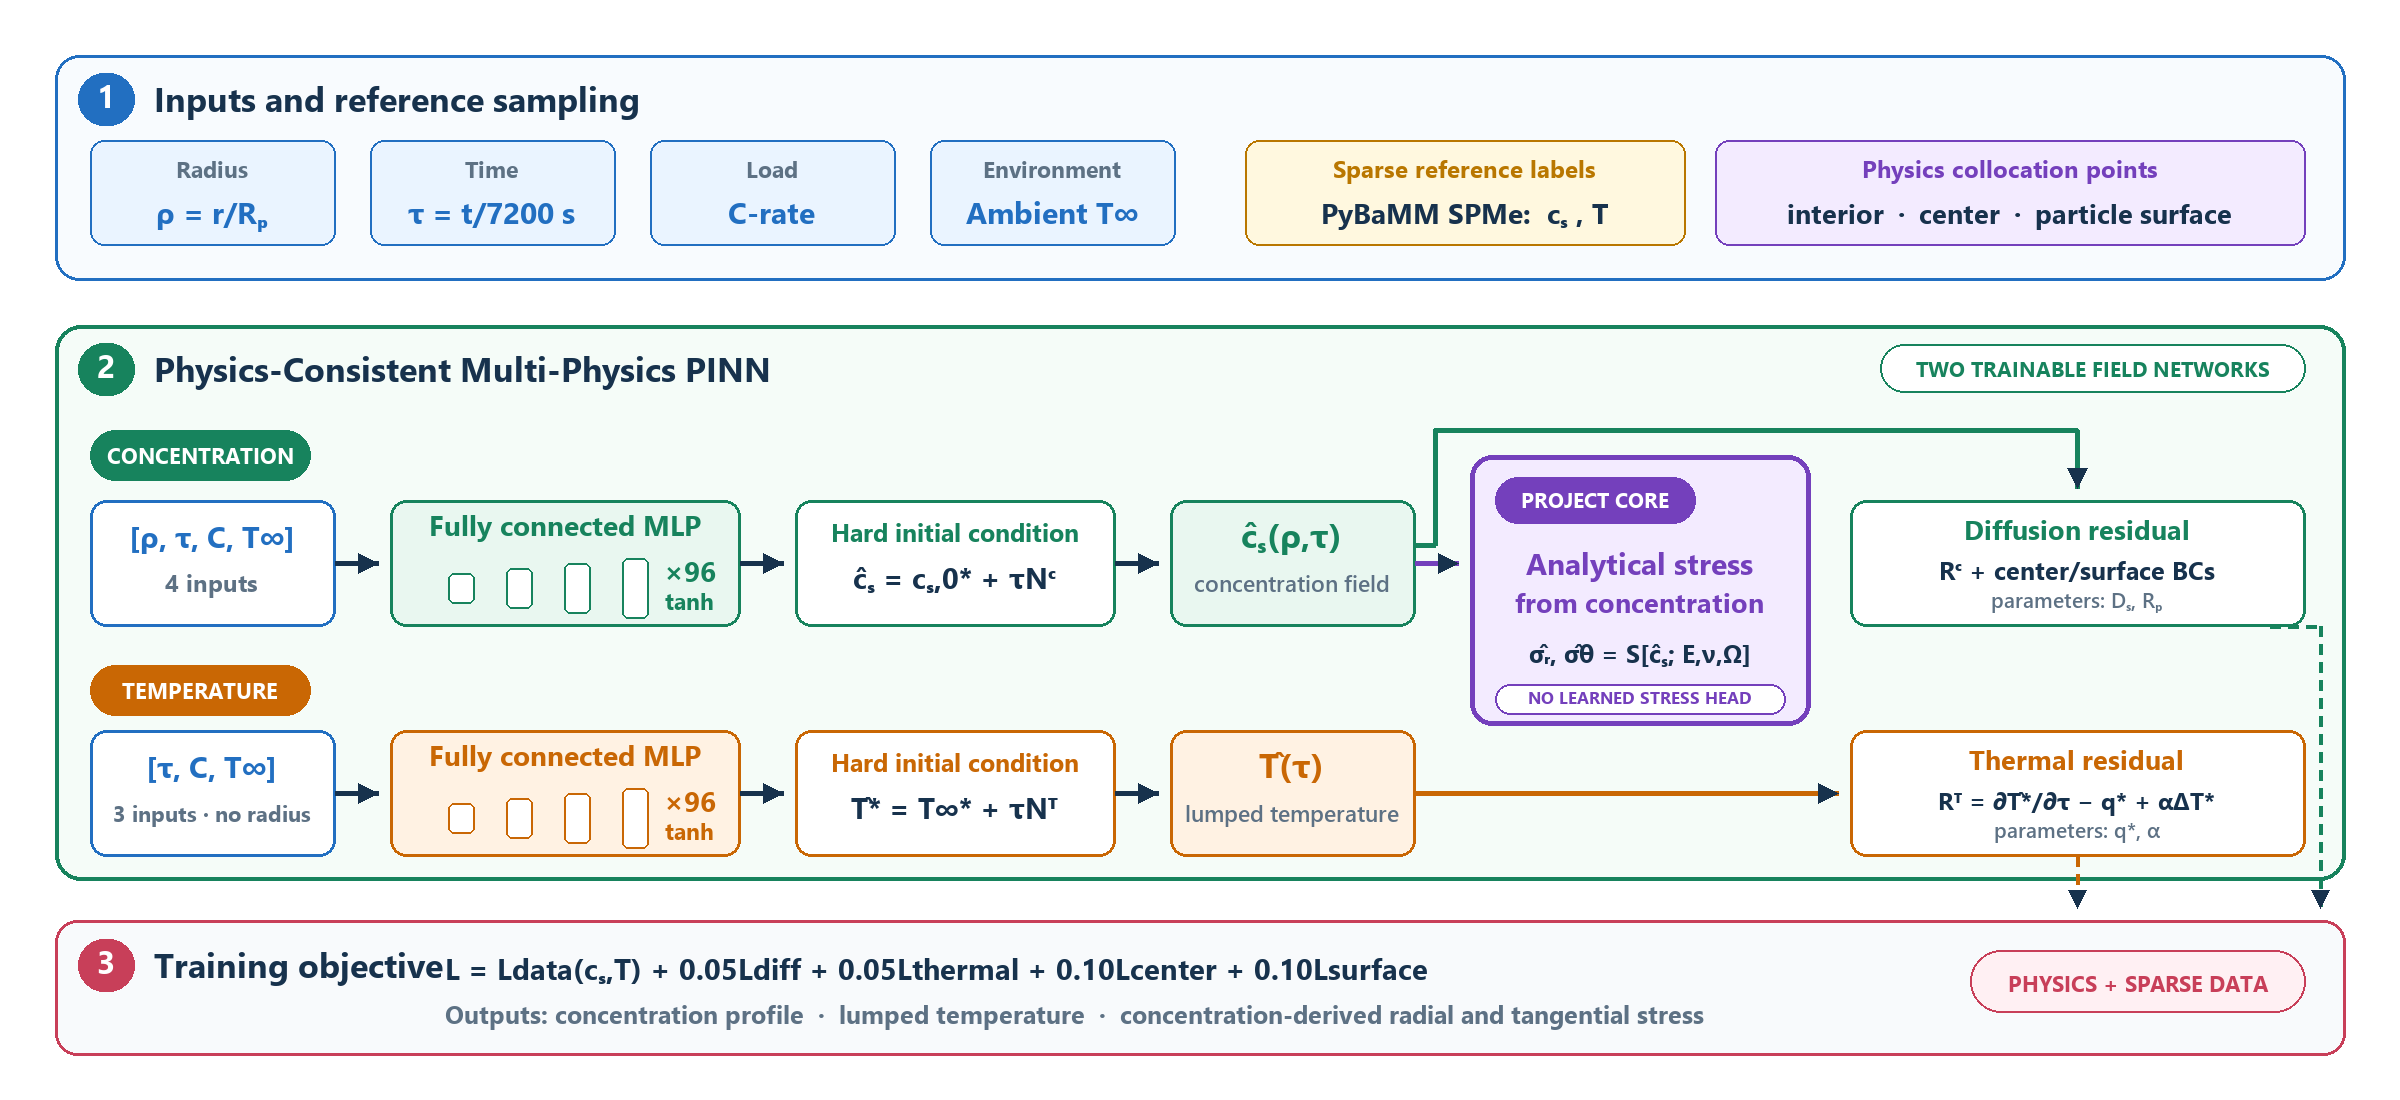
\includegraphics[width=\textwidth]{pinn_architecture.png}
\caption{Proposed \modelname{} architecture. The temperature branch matches the lumped thermal assumption, while stress is an analytical function of predicted concentration.}
\label{fig:architecture}
\end{figure*}

\subsection{Physics Residuals}
Automatic differentiation evaluates the time and radius derivatives. After substituting the normalized coordinates, the diffusion mismatch becomes
\begin{equation}
\mathcal{R}_{c}=\frac{\partial \widehat c_s}{\partial \tau}
-\frac{D_s t_{\mathrm{ref}}}{R_p^2}\left(
\frac{\partial^2\widehat c_s}{\partial \bar r^2}
+\frac{2}{\bar r}\frac{\partial\widehat c_s}{\partial \bar r}\right).
\label{eq:rc}
\end{equation}
Interior samples begin at $\bar r=10^{-3}$ so the spherical $2/\bar r$ term is finite. A separate boundary term enforces the derivative at the true center. The energy-balance mismatch is
\begin{equation}
\mathcal{R}_{T}=\rho_{\mathrm{eff}}c_{p,\mathrm{eff}}
\frac{1}{t_{\mathrm{ref}}}\frac{\partial\widehat T}{\partial\tau}
-q_{\mathrm{gen}}+\frac{hA_{\mathrm{cool}}}{V_{\mathrm{cell}}}
(\widehat T-T_{\mathrm{amb}}).
\label{eq:rt}
\end{equation}
The normalized physics loss is
\begin{equation}
\mathcal{L}_{\mathrm{phys}}=\|\mathcal{R}_c\|_2^2
+\|\widetilde{\mathcal{R}}_T\|_2^2
+\|\mathcal{R}_{r=0}\|_2^2+\|\mathcal{R}_{r=R_p}\|_2^2,
\label{eq:lphys}
\end{equation}
The tilde indicates division by $\rho c_p\Delta T_{\mathrm{scale}}/t_{\mathrm{ref}}$. This nondimensionalization keeps the thermal term from outweighing the other residuals solely because of its units.

\subsection{Supervised and Total Loss}
At labeled points $\mathcal{D}_L$, training compares normalized concentration and temperature rise:
\begin{equation}
\mathcal{L}_{\mathrm{data}}=\frac{1}{|\mathcal{D}_L|}
\sum_{i\in\mathcal{D}_L}\left[(\widehat c_{s,i}^{\,*}-c_{s,i}^{*})^2
+(\widehat{\Delta T}_i/50-\Delta T_i/50)^2\right].
\label{eq:ldata}
\end{equation}
The two terms are added with the weights shown in Fig.~\ref{fig:architecture}. Both comparison models retain explicit radial- and tangential-stress outputs. The proposed network has no stress target in its supervised loss because mechanics is evaluated from $\widehat c_s$.

\subsection{Reproducible implementation}
PyBaMM solves each C-rate and ambient-temperature pair as a separate simulation. The export contains physical time, negative-electrode interfacial current, heat generation, average temperature, and particle concentration on one time--radius grid. Training and evaluation use the following sequence:
\begin{enumerate}
    \item reserve complete operating conditions for training, validation, and testing;
    \item estimate normalization constants from training conditions and keep an unscaled copy of every variable used in a residual;
    \item sample labeled rows and physics collocation points independently within each training trajectory;
    \item optimize with Adam, retaining the checkpoint with the smallest validation objective and applying the stated patience rule; and
    \item reload that checkpoint, evaluate the untouched test conditions once, compute stress from concentration, and write the metrics.
\end{enumerate}
All variants receive identical condition partitions and identical labeled indices for a given seed. Physics points are resampled during optimization, whereas validation and test grids do not change. Each checkpoint is accompanied by the software version, parameter set, seed, label budget, chosen epoch, elapsed time, and trainable-parameter count.

The stress calculation needs an integral along particle radius. For each time and operating condition, predicted concentrations are ordered by radius and integrated with the cumulative trapezoidal rule. At the center, the limiting expression is evaluated directly. Replacing $r^3$ by an arbitrary small denominator would distort the center stress and can also change the reported peak.

\section{Experimental Methodology}
\subsection{Reference data and condition split}
The reference set contains constant-current SPMe discharges with lumped thermal coupling and Chen2020 parameters. A run stops at 2.5~V. We retain 100 time samples and 25 radial samples from each run. Training uses the Cartesian product of C-rates $\{0.5,1.0,1.5,2.0\}$ and ambient temperatures $\{10,25,35\}^{\circ}$C. Validation uses C-rates $\{0.75,1.75\}$ at $\{15,30\}^{\circ}$C. The two final test cases are 1.25C discharges at $20^{\circ}$C and $32.5^{\circ}$C. In total, the dataset has 18 trajectories and 45,000 radius--time records.

No trajectory is divided across subsets. Validation data determine early stopping and checkpoint choice; the test trajectories are read only after fitting has ended. Figure~\ref{fig:design} shows the sampled operating envelope and the matched ablation design.

\begin{figure*}[!b]
\centering
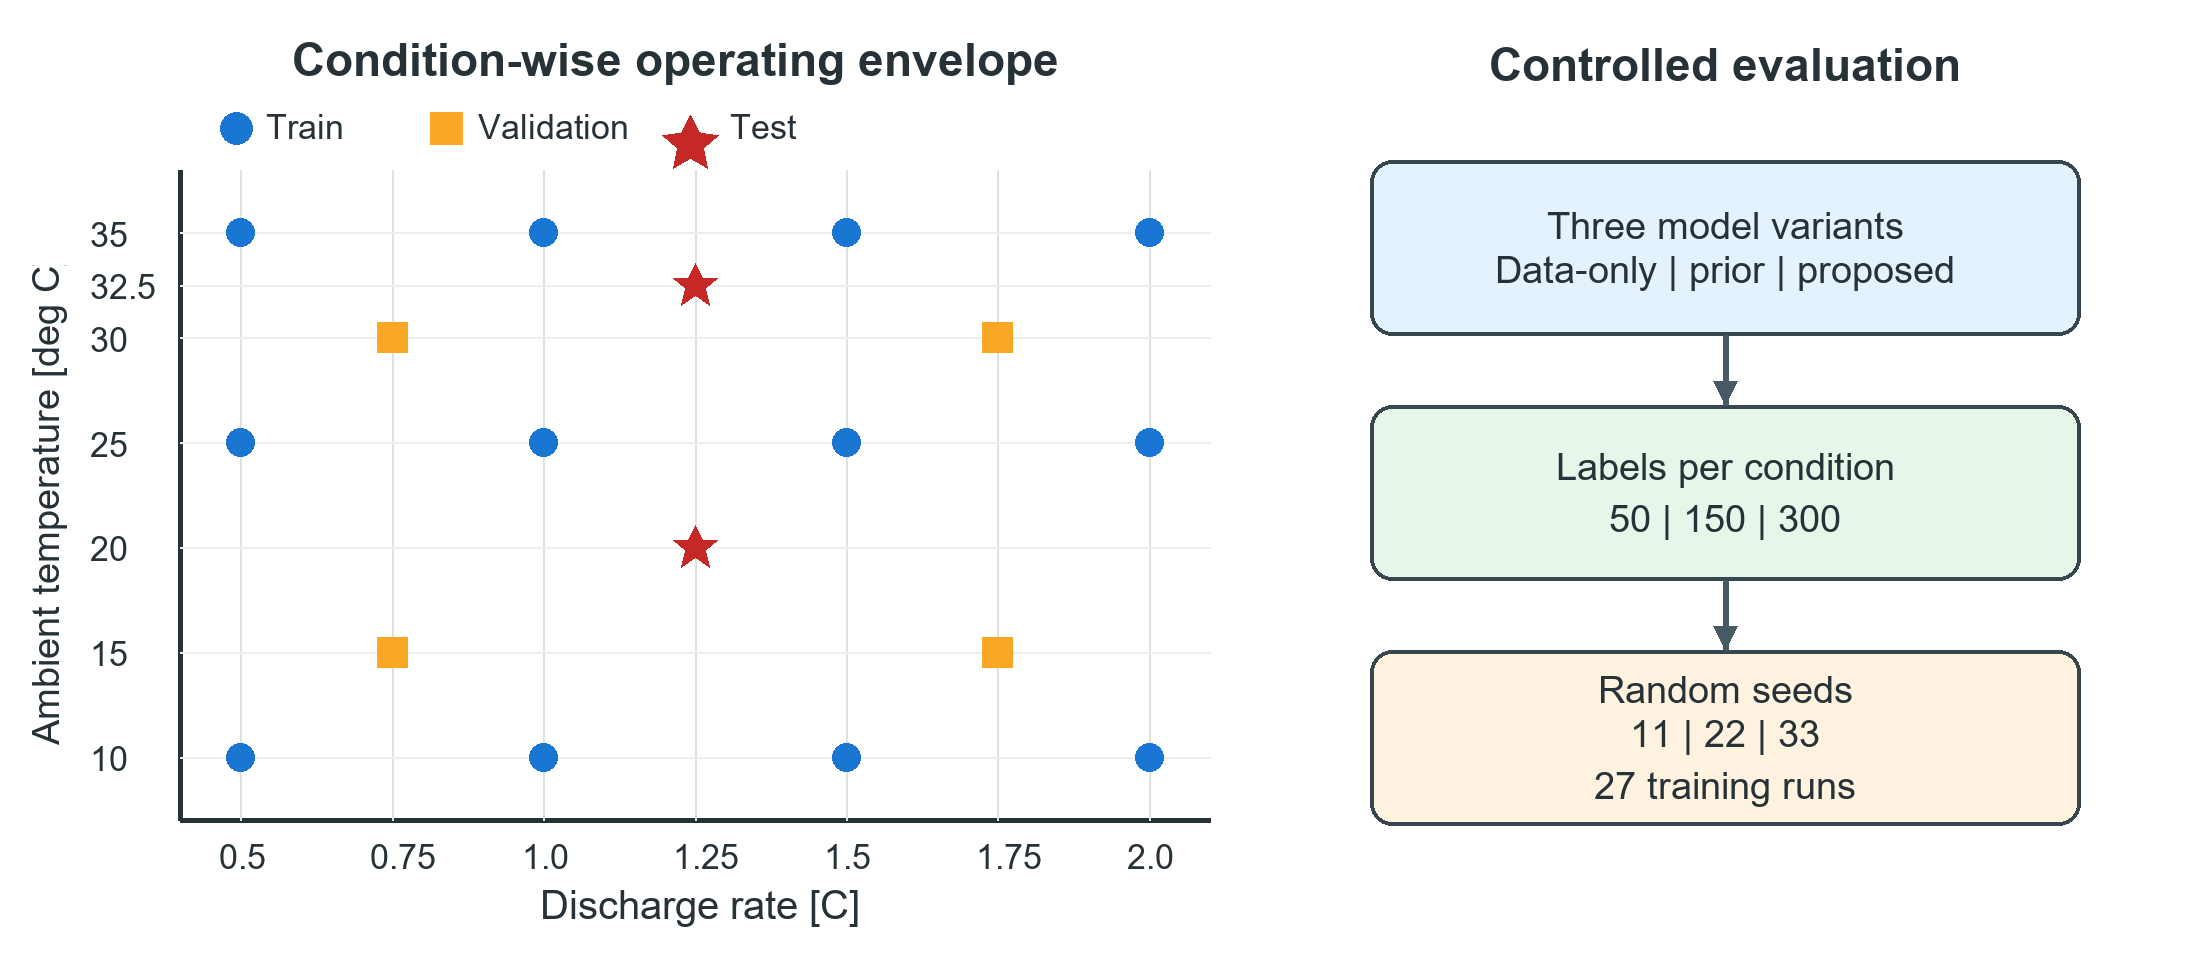
\includegraphics[width=0.96\textwidth]{experimental_design.png}
\caption{Operating conditions and matched comparisons. Model variants differ in formulation, while partitions, label counts, and random seeds remain fixed.}
\label{fig:design}
\end{figure*}

\subsection{Models and optimization settings}
Three formulations are trained. The \textbf{data-only} network reproduces the earlier four-output design and fits concentration, temperature, radial stress, and tangential stress. The \textbf{prior-style PINN} keeps those outputs and adds diffusion, thermal, boundary, and mechanical-equilibrium penalties. The \textbf{proposed \modelname} removes both stress heads and generates stress from its concentration field.

For every formulation, each training trajectory contributes either 50, 150, or 300 labeled records. Seeds 11, 22, and 33 give 27 primary runs. Adam starts at $10^{-3}$; gradients are clipped at norm 10. Training ends at 2500 epochs or after 350 epochs without validation improvement. Each training condition supplies 900 interior and 120 boundary collocation points. Test evaluation always uses the saved validation-selected state.

\begin{table}[t]
\centering
\caption{Full Experimental Configuration}
\label{tab:config}
\footnotesize
\setlength{\tabcolsep}{3.5pt}
\begin{tabular}{p{0.43\columnwidth}p{0.50\columnwidth}}
\toprule
Item & Value \\
\midrule
Reference model & PyBaMM SPMe, lumped thermal \\
Parameter set & Chen2020 (LG M50) \\
Cutoff voltage & 2.5 V \\
Radial/time samples & 25 / 100 per condition \\
PINN hidden layers & $4\times96$, tanh \\
Optimizer & Adam, $10^{-3}$ \\
Maximum epochs / patience & 2500 / 350 \\
Interior collocation points & 900 per train condition \\
Boundary points & 120 per train condition \\
Label budgets & 50, 150, 300 \\
Random seeds & 11, 22, 33 \\
Mechanical constants & $E=15$ GPa, $\nu=0.30$ \\
Partial molar volume & $\Omega=3.497\times10^{-6}$ m$^3$ mol$^{-1}$ \\
\bottomrule
\end{tabular}
\end{table}

\subsection{Controlled comparisons}
The first comparison, data-only versus prior-style PINN, tests whether the added residuals help the existing four-output network. The second comparison changes two linked design choices: it replaces trainable stress outputs with the analytical operator and removes radius from the temperature branch. Results from this pair therefore measure the revised architecture as a whole. They cannot attribute every change to mechanics alone. Repeating both comparisons at 50, 150, and 300 labels reveals how their behavior changes as supervision becomes less sparse.

If computational time permits, three diagnostic runs can separate these effects: omit the thermal residual but keep temperature labels; apply the stress operator to concentration from the data-only network; and replace only the stress heads in the prior-style PINN while leaving its temperature input unchanged. These runs aid diagnosis but do not replace the predeclared three-model experiment.

\subsection{Evaluation measures}
One score cannot describe a coupled field surrogate. We therefore report nine measures spanning prediction, physical checks, and runtime. For any reference field $y$ and prediction $\widehat y$ at $N$ locations,
\begin{align}
\operatorname{RMSE}(y)&=\sqrt{\frac{1}{N}\sum_{i=1}^{N}(\widehat y_i-y_i)^2},
\label{eq:rmse}\\
\operatorname{Rel}L_2(y)&=\frac{\|\widehat{\mathbf y}-\mathbf y\|_2}{\|\mathbf y\|_2}.
\label{eq:rell2}
\end{align}
The nine reported quantities are concentration relative $L_2$ error, surface-concentration MAE, temperature-rise RMSE, largest absolute temperature-rise error, tangential-stress RMSE, peak tensile-stress error, particle mass-balance RMSE, concentration--stress consistency RMSE, and median speedup relative to SPMe. MAPE is unsuitable for stress because the denominator approaches or crosses zero. Temperature scores use rise above ambient; division by absolute Kelvin temperature would make meaningful thermal deviations appear artificially small.

As a separate conservation check, the particle-average concentration must satisfy

\begin{equation}
\mathcal{R}_{m}=\frac{d\bar c_s}{dt}+\frac{3j_n}{FR_p},\quad
\bar c_s=\frac{3}{R_p^3}\int_0^{R_p}c_s(r,t)r^2\,dr.
\label{eq:mass}
\end{equation}
For the coupling check, stress is recomputed from each model's concentration and compared with that model's stress output. In the proposed architecture these two quantities are the same construction, leaving only floating-point and quadrature error. Results include the seed mean, sample standard deviation, and the poorer of the two held-out conditions. Relative change from the prior-style model is
\begin{equation}
\Delta_m(\%)=100\frac{m_{\mathrm{prior}}-m_{\mathrm{proposed}}}
{|m_{\mathrm{prior}}|+\epsilon},
\label{eq:gap}
\end{equation}
A positive $\Delta_m$ means that the revised model has the smaller error.

\subsubsection{Inference latency and solver speedup}
Runtime is measured with the same held-out query batch, numerical precision, and computer for both methods. Let $\widetilde t_{\mathrm{PINN}}$ and $\widetilde t_{\mathrm{SPMe}}$ be the median times across repeated blocks. We define
\begin{equation}
S_{\mathrm{lat}}=\frac{\widetilde t_{\mathrm{SPMe}}}{\widetilde t_{\mathrm{PINN}}}.
\label{eq:speedup}
\end{equation}
The timing loop performs 100 warm-up calls and synchronizes pending operations before recording the median and 95th percentile. A ratio above one favors PINN inference. Training duration is listed separately because it is a one-time cost and is not part of per-query latency.

\begin{figure}[!b]
\centering
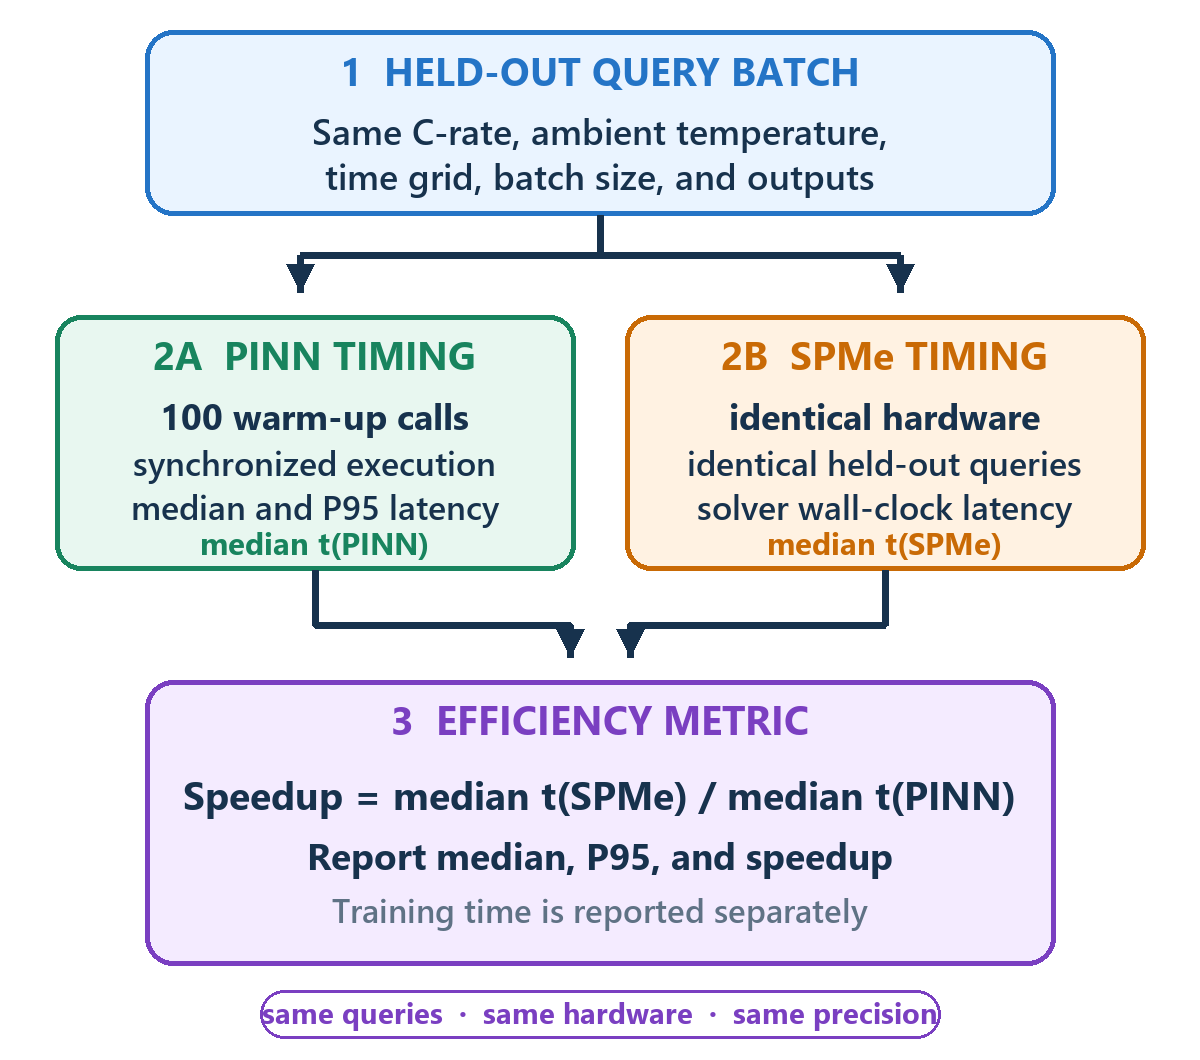
\includegraphics[width=0.98\columnwidth]{inference_efficiency_protocol_column.png}
\caption{Timing procedure for the PINN and SPMe reference solver on one held-out query batch.}
\label{fig:latency_protocol}
\end{figure}

\subsection{Aggregation and decision rule}
Metrics are first computed for each test condition and seed. For a given model and label budget, the main summary averages the two conditions within each seed and then reports the mean and sample standard deviation over the three seeds. The worse test condition is retained as a separate column; an average can otherwise hide a temperature-specific failure. With only three seeds, the standard deviation describes run-to-run variation and is not treated as a significance test.

Support for the hypothesis requires more than a zero coupling residual. The revised model must remove the designed concentration--stress mismatch, avoid a material increase in stress error, and keep concentration and temperature accuracy comparable across label budgets. Timing claims are valid only under the fixed procedure in Fig.~\ref{fig:latency_protocol}. Parameter count and training duration are supporting resource measures.

\section{Results and Discussion}
\subsection{Result-reporting rule}
Table~\ref{tab:results} reads values produced by the notebook summaries \texttt{paper\_metrics\_summary.csv} and \texttt{variation\_gap\_vs\_previous.csv}. Placeholder text is retained in this draft because the complete three-seed experiment has not yet been inserted. A submission version must run with \texttt{quick\_mode=False} and replace every macro at the start of the source with the measured mean and standard deviation. No numerical result is inferred from an incomplete run.

\begin{table*}[t]
\centering
\caption{Held-Out Test Performance at 300 Labels per Training Condition (Mean $\pm$ Standard Deviation Across Three Seeds)}
\label{tab:results}
\footnotesize
\resizebox{0.98\textwidth}{!}{%
\begin{tabular}{lccccc}
\toprule
Model & Concentration Rel-$L_2$ & Temp.-rise RMSE [K] & Tangential-stress RMSE [MPa] & Mass-balance RMSE [mol m$^{-3}$ s$^{-1}$] & Median speedup [$\times$] \\
\midrule
Data-only & \DataC & \DataT & \DataStress & \DataMass & \DataSpeed \\
Prior-style PINN & \PriorC & \PriorT & \PriorStress & \PriorMass & \PriorSpeed \\
Proposed \modelname & \ProposedC & \ProposedT & \ProposedStress & \ProposedMass & \ProposedSpeed \\
\bottomrule
\end{tabular}
}
\end{table*}

\subsection{Plots and traceability}
The notebook exports plots of error against label count, surface concentration, temperature rise, and both stress components. A separate panel shows the mass-balance residual. Each plot names the held-out condition and seed aggregation. Scalar scores provide a compact comparison, while trajectories reveal timing offsets, boundary errors, and short stress peaks that an average may hide.

All summaries are built from the same condition-level results file. Before aggregation, the script checks for the 27 expected runs, verifies that condition groups do not overlap, and confirms three seeds for each reported mean. An unsuccessful run remains visible as incomplete rather than being dropped from the denominator.

\subsection{Questions answered by the experiment}
The experiment tests whether residual training helps when labels are scarce and whether the analytical mechanics layer improves agreement between concentration and stress without sacrificing the two learned fields. The evidence must include all seeds, both test conditions, peak and field stress errors, and the independent conservation calculation. The test points lie inside the sampled C-rate and ambient-temperature range. They say nothing about charging, arbitrary drive cycles, different chemistries, or extreme temperatures.

\subsection{Expected physical behavior}
During discharge, reaction at the particle surface can create a radial concentration gradient and hence diffusion-induced stress. A spatially uniform profile gives zero stress under Eqs.~\eqref{eq:sr} and \eqref{eq:st}; faster discharge is expected to increase transient nonuniformity. Equation~\eqref{eq:thermal} links temperature rise to generated heat and convective removal. Unlike parameter-inference PINNs \cite{hassanaly2024part1,hassanaly2024part2}, aging-oriented models \cite{wei2026etm}, and life-cycle temperature predictors \cite{wang2023temperature}, this experiment evaluates within-discharge agreement between electrochemical and mechanical fields. These physical expectations are checks on the measured curves, not substitutes for them.

\section{Limitations and Threats to Validity}
Every target in this study is simulated. Agreement with PyBaMM shows that the surrogate reproduces the selected SPMe configuration; it does not constitute experimental validation. The model represents one negative-electrode particle, one cell-average temperature, fixed material properties, and constant-current discharge. It omits through-thickness thermal gradients, spatially varying electrode stress, plastic deformation, binder behavior, fracture initiation, and two-way stress--diffusion feedback.

The elastic constants are literature values rather than measurements from the modeled LG M50 cell. The resulting stress should be interpreted as a model-derived indicator. Chen2020 parameters were assembled from multiscale experiments, but a parameter set remains an input to the mathematical model rather than proof of every internal property of a particular cell \cite{chen2020parameterization}.

Heat-generation histories also come from the SPMe reference. The neural network interpolates within the selected constant-current conditions and has not been tested with an arbitrary current waveform. PINN optimization adds another limitation: data and residual terms can produce gradients of very different sizes. Repeated seeds and independent residual calculations expose some unstable fits but cannot remove error in the governing assumptions.

The study makes no aging claim. PyBaMM can represent SEI growth, plating, active-material loss, and cracking \cite{sulzer2021pybamm}, but a credible degradation experiment would also need cycling schedules, health or capacity targets, degradation parameters, and held-out cells or profiles. Stress may later act as an input to such a model; it is not interchangeable with degradation.

\subsection{Sensitivity and numerical uncertainty}
Equations~\eqref{eq:sr} and \eqref{eq:st} scale stress by $E\Omega/(1-\nu)$. Errors in $E$ or $\Omega$ can therefore dominate the mechanical result even if concentration is accurate. The planned sensitivity calculation passes each stored concentration field through the operator after changing $E$ and $\Omega$ separately by $\pm20\%$. It records the change in peak stress without retraining. Because $D_s$ is fixed during fitting, conclusions apply to the selected Chen2020 diffusivity.

The radial integral is repeated with 25, 50, and 100 grid points. Peak stress and mass-balance error should approach stable values as the grid is refined; otherwise the reported difference may be a quadrature artifact.

\subsection{Failure analysis}
The saved histories allow failures to be assigned to specific stages. High concentration error with a small PDE residual suggests a boundary, scaling, or initial-condition problem. Low label error with a large off-grid residual points to poor physical generalization. If concentration is accurate but stress is not, the elastic constants or radial integration should be checked. A nearly constant temperature bias suggests heat capacity or heat generation, whereas an error that changes with ambient temperature points toward the cooling term.

Non-finite losses, very early checkpoints, and runs still improving at epoch 2500 are reported with their seeds rather than replaced. The held-out cases measure interpolation only. Robustness would require additional tests with noise, parameter shifts, and current profiles. A small residual confirms agreement with the equations imposed during training; it cannot establish that those equations include every relevant process.

\balance
\section{Conclusion}
This work revises a battery PINN so that its mechanical field is tied directly to its electrochemical field. The trainable outputs are particle concentration and lumped temperature. Radial and tangential stresses follow from the concentration integral, while diffusion and energy-balance residuals regularize the learned fields. The evaluation keeps complete operating conditions separate and repeats matched model variants across label budgets and seeds.

The final claim depends on the full experiment. The redesign is useful only if it removes concentration--stress disagreement without materially worsening stress, concentration, or temperature error. If consistency improves but prediction does not, the next step is to improve concentration learning or calibrate the mechanical constants rather than claim success from the architectural identity alone. Experimental cells, dynamic-current profiles, and cycling data are needed before extending the conclusions to degradation or battery health.

\section*{Data and Code Availability}
The project notebook generates the PyBaMM trajectories, trains the three formulations, and writes checkpoints, per-condition metrics, and label-budget comparisons. An archived release should include the data, weights, software versions, and random seeds listed in Table~\ref{tab:config}.

\section*{Acknowledgment}
The authors acknowledge the Department of Computer Science and Engineering, KPR Institute of Engineering and Technology, for supporting this project.

\begin{thebibliography}{00}
\setlength{\itemsep}{0pt}
\bibitem{doyle1993dfn}
M. Doyle, T. F. Fuller, and J. Newman, ``Modeling of galvanostatic charge and discharge of the lithium/polymer/insertion cell,'' \emph{J. Electrochem. Soc.}, vol. 140, no. 6, pp. 1526--1533, 1993, doi: 10.1149/1.2221597.

\bibitem{marquis2019spme}
S. G. Marquis, V. Sulzer, R. Timms, C. P. Please, and S. J. Chapman, ``An asymptotic derivation of a single particle model with electrolyte,'' \emph{J. Electrochem. Soc.}, vol. 166, no. 15, pp. A3693--A3706, 2019, doi: 10.1149/2.0341915jes.

\bibitem{richardson2020gspm}
G. Richardson, I. Korotkin, R. Ranom, M. J. Castle, and J. M. Foster, ``Generalised single particle models for high-rate operation of graded lithium-ion electrodes: Systematic derivation and validation,'' \emph{Electrochim. Acta}, vol. 339, art. 135862, 2020, doi: 10.1016/j.electacta.2020.135862.

\bibitem{planella2022continuum}
F. Brosa Planella \emph{et al.}, ``A continuum of physics-based lithium-ion battery models reviewed,'' \emph{Prog. Energy}, vol. 4, no. 4, art. 042003, 2022, doi: 10.1088/2516-1083/ac7d31.

\bibitem{raissi2019pinn}
M. Raissi, P. Perdikaris, and G. E. Karniadakis, ``Physics-informed neural networks: A deep learning framework for solving forward and inverse problems involving nonlinear partial differential equations,'' \emph{J. Comput. Phys.}, vol. 378, pp. 686--707, 2019, doi: 10.1016/j.jcp.2018.10.045.

\bibitem{hassanaly2024part1}
M. Hassanaly \emph{et al.}, ``PINN surrogate of Li-ion battery models for parameter inference, Part I: Implementation and multi-fidelity hierarchies for the single-particle model,'' \emph{J. Energy Storage}, vol. 98, art. 113103, 2024, doi: 10.1016/j.est.2024.113103.

\bibitem{hassanaly2024part2}
M. Hassanaly \emph{et al.}, ``PINN surrogate of Li-ion battery models for parameter inference, Part II: Regularization and application of the pseudo-2D model,'' \emph{J. Energy Storage}, vol. 98, art. 113104, 2024, doi: 10.1016/j.est.2024.113104.

\bibitem{wang2023temperature}
Y. Wang, C. Xiong, Y. Wang, P. Xu, C. Ju, J. Shi, G. Yang, and J. Chu, ``Temperature state prediction for lithium-ion batteries based on improved physics informed neural networks,'' \emph{J. Energy Storage}, vol. 73, art. 108863, 2023, doi: 10.1016/j.est.2023.108863.

\bibitem{wang2024parameter}
J. Wang, Q. Peng, J. Meng, T. Liu, J. Peng, and R. Teodorescu, ``A physics-informed neural network approach to parameter estimation of lithium-ion battery electrochemical model,'' \emph{J. Power Sources}, vol. 621, art. 235271, 2024, doi: 10.1016/j.jpowsour.2024.235271.

\bibitem{wei2026etm}
Y. Wei, K. Liu, J. Rui, and Q. Zhao, ``Integrating electrochemical-thermal-mechanical physical informed neural network framework for lithium-ion batteries state of health estimation,'' \emph{Energy AI}, vol. 24, art. 100713, 2026, doi: 10.1016/j.egyai.2026.100713.

\bibitem{cheng2009stress}
Y.-T. Cheng and M. W. Verbrugge, ``Evolution of stress within a spherical insertion electrode particle under potentiostatic and galvanostatic operation,'' \emph{J. Power Sources}, vol. 190, no. 2, pp. 453--460, 2009, doi: 10.1016/j.jpowsour.2009.01.021.

\bibitem{zhuang2026spm}
Y. Zhuang, Y. Zheng, Y. Che, and R. Teodorescu, ``Physics-informed neural network surrogate modeling of single particle model for lithium-ion batteries,'' arXiv:2601.01466, 2026.

\bibitem{fu2024spacecraft}
H. Fu, Z. Liu, K. Cui, Q. Du, J. Wang, and D. Shi, ``Physics-informed neural network for spacecraft lithium-ion battery modeling and health diagnosis,'' \emph{IEEE/ASME Trans. Mechatronics}, vol. 29, no. 5, pp. 3546--3555, 2024, doi: 10.1109/TMECH.2023.3348519.

\bibitem{dang2024soc}
L. Dang, J. Yang, M. Liu, and B. D. Chen, ``Differential equation-informed neural networks for state-of-charge estimation,'' \emph{IEEE Trans. Instrum. Meas.}, vol. 73, pp. 1--12, 2024, doi: 10.1109/TIM.2023.3334377.

\bibitem{ye2024soh}
J. Ye, Q. Xie, M. Lin, and J. Wu, ``A method for estimating the state of health of lithium-ion batteries based on physics-informed neural network,'' \emph{Energy}, vol. 294, art. 130828, 2024, doi: 10.1016/j.energy.2024.130828.

\bibitem{jiang2025heatmap}
Y. Jiang, Z. Liu, P. Kabirzadeh, Y. Wu, Y. Li, N. Miljkovic, and P. Wang, ``Multi-fidelity physics-informed convolutional neural network for heat map prediction of battery packs,'' \emph{Reliab. Eng. Syst. Saf.}, vol. 256, art. 110752, 2025, doi: 10.1016/j.ress.2024.110752.

\bibitem{tian2025generic}
A. Tian, L. He, T. Ding, K. Dong, Y. Wang, and J. Jiang, ``A generic physics-informed neural network framework for lithium-ion batteries state of health estimation,'' \emph{Energy}, vol. 332, art. 137215, 2025, doi: 10.1016/j.energy.2025.137215.

\bibitem{xiong2025diagnostics}
R. Xiong, Y. He, Y. Sun, Y. Jia, and W. Shen, ``Enhanced electrode-level diagnostics for lithium-ion battery degradation using physics-informed neural networks,'' \emph{J. Energy Chem.}, vol. 104, pp. 618--627, 2025, doi: 10.1016/j.jechem.2025.01.019.

\bibitem{chen2025smallsample}
L. Chen \emph{et al.}, ``Physics-informed neural networks for small sample state of health estimation of lithium-ion batteries,'' \emph{J. Energy Storage}, vol. 122, art. 116559, 2025, doi: 10.1016/j.est.2025.116559.

\bibitem{luo2025hybrid}
Y. Luo, S. Ju, P. Li, and H. Zhang, ``A method for estimating lithium-ion battery state of health based on physics-informed hybrid neural network,'' \emph{Electrochim. Acta}, vol. 525, art. 146110, 2025, doi: 10.1016/j.electacta.2025.146110.

\bibitem{lyu2024digitaltwin}
C. Lyu, S. Xu, J. Li, and M. Pecht, ``Digital twin modeling method for lithium-ion batteries based on data-mechanism fusion driving,'' \emph{Green Energy Intell. Transp.}, vol. 3, no. 5, art. 100162, 2024, doi: 10.1016/j.geits.2024.100162.

\bibitem{christensen2006fracture}
J. Christensen and J. Newman, ``A mathematical model of stress generation and fracture in lithium manganese oxide,'' \emph{J. Electrochem. Soc.}, vol. 153, no. 6, pp. A1019--A1030, 2006, doi: 10.1149/1.2185287.

\bibitem{xu2016electrochemomechanics}
R. Xu and K. Zhao, ``Electrochemomechanics of electrodes in Li-ion batteries: A review,'' \emph{J. Electrochem. Energy Convers. Storage}, vol. 13, no. 3, art. 030803, 2016, doi: 10.1115/1.4035310.

\bibitem{sulzer2021pybamm}
V. Sulzer, S. G. Marquis, R. Timms, M. Robinson, and S. J. Chapman, ``Python Battery Mathematical Modelling (PyBaMM),'' \emph{J. Open Res. Softw.}, vol. 9, no. 1, art. 14, 2021, doi: 10.5334/jors.309.

\bibitem{chen2020parameterization}
C.-H. Chen, F. Brosa Planella, K. O'Regan, D. Gastol, W. D. Widanage, and E. Kendrick, ``Development of experimental techniques for parameterization of multi-scale lithium-ion battery models,'' \emph{J. Electrochem. Soc.}, vol. 167, no. 8, art. 080534, 2020, doi: 10.1149/1945-7111/ab9050.

\bibitem{bernardi1985energy}
D. Bernardi, E. Pawlikowski, and J. Newman, ``A general energy balance for battery systems,'' \emph{J. Electrochem. Soc.}, vol. 132, no. 1, pp. 5--12, 1985, doi: 10.1149/1.2113792.

\end{thebibliography}

\end{document}


